
%-=-=-=-=-=-=-=-=-=-=-=-=-=-=-=-=-=-=-=-=-=-=-=-=
%
%        LOADING DOCUMENT
%
%-=-=-=-=-=-=-=-=-=-=-=-=-=-=-=-=-=-=-=-=-=-=-=-=

\documentclass[compress]{beamer}
\usetheme{sthlm}

%-=-=-=-=-=-=-=-=-=-=-=-=-=-=-=-=-=-=-=-=-=-=-=-=
%        LOADING BEAMER PACKAGES
%-=-=-=-=-=-=-=-=-=-=-=-=-=-=-=-=-=-=-=-=-=-=-=-=

\usepackage{
booktabs,
datetime,
dtklogos,
graphicx,
multicol,
pgfplots,
ragged2e,
tabularx,
tikz,
wasysym
}

\pgfplotsset{compat=1.8}
\usepackage[T1]{fontenc}
\usepackage{newpxtext,newpxmath}
\usepackage{pifont}% http://ctan.org/pkg/pifont
\usepackage[utf8x]{inputenc}

\usepackage{multicol}
\usepackage{caption}
\usepackage{pgfgantt}
\usepackage{graphicx} % Allows including images
\usepackage{booktabs} % Allows the use of \toprule, \midrule and \bottomrule in tables

\usepackage{listings}
\usepackage{color, colortbl}
\newcommand{\cmark}{\color{green}\ding{51}}%
\newcommand{\xmark}{\color{red}\ding{55}}%

\lstset{ %
language=[LaTeX]TeX,
basicstyle=\normalsize\ttfamily,
keywordstyle=,
numbers=left,
numberstyle=\tiny\ttfamily,
stepnumber=1,
showspaces=false,
showstringspaces=false,
showtabs=false,
breaklines=true,
frame=tb,
framerule=0.5pt,
tabsize=4,
framexleftmargin=0.5em,
framexrightmargin=0.5em,
xleftmargin=0.5em,
xrightmargin=0.5em
}

%-=-=-=-=-=-=-=-=-=-=-=-=-=-=-=-=-=-=-=-=-=-=-=-=
%        LOADING TIKZ LIBRARIES
%-=-=-=-=-=-=-=-=-=-=-=-=-=-=-=-=-=-=-=-=-=-=-=-=

\usetikzlibrary{
backgrounds,
mindmap
}

%-=-=-=-=-=-=-=-=-=-=-=-=-=-=-=-=-=-=-=-=-=-=-=-=
%        BEAMER OPTIONS
%-=-=-=-=-=-=-=-=-=-=-=-=-=-=-=-=-=-=-=-=-=-=-=-=

\setbeameroption{show notes}

%-=-=-=-=-=-=-=-=-=-=-=-=-=-=-=-=-=-=-=-=-=-=-=-=
%        BEAMER COMMANDS
%-=-=-=-=-=-=-=-=-=-=-=-=-=-=-=-=-=-=-=-=-=-=-=-=


%-=-=-=-=-=-=-=-=-=-=-=-=-=-=-=-=-=-=-=-=-=-=-=-=
%
%	PRESENTATION INFORMATION
%
%-=-=-=-=-=-=-=-=-=-=-=-=-=-=-=-=-=-=-=-=-=-=-=-=
\usepackage{tikz}
\usepackage{pgf}



\logo{
\includegraphics[height=1.5cm]{logo.pdf}}
\newcommand{\nologo}{\setbeamertemplate{logo}{}}
\definecolor{Gray}{gray}{0.9}
\newcommand{\myquote}[2]{\begin{exampleblock}{}{\large ``#1''}\vskip5mm\hspace*\fill{\small--- #2}\end{exampleblock}}
%----------------------------------------------------------------------------------------
%	TITLE PAGE
%----------------------------------------------------------------------------------------

\title{Hyper-linked Communications} 
\subtitle{WebRTC enabled asynchronous collaboration}


\author{Henrique Rocha} % Your name
\institute[IST] % Your institution as it will appear on the bottom of every slide, may be shorthand to save space
{
Instituto Superior Técnico \\
Universidade de Lisboa \\ % Your institution for the title page
\medskip
\textit{henrique.rocha@tecnico.ulisboa.pt}\\ % Your email address
\small

Advisor: Ricardo Pereira \\
Co-Advisor: Paulo Chainho \\
}
\date{\today} % Date, can be changed to a custom date

\begin{document}
{
\nologo
\begin{frame}
\maketitle % Print the title page as the first slide

\end{frame}
}

\begin{frame}[t]
\frametitle{Overview} 
\tableofcontents[hidesubsections]


\end{frame}

%----------------------------------------------------------------------------------------
%	PRESENTATION SLIDES
%----------------------------------------------------------------------------------------

%------------------------------------------------

\section{Introduction}\label{intro}

%\begin{frame}[t,shrink]
%\frametitle{Introduction} 
%\tableofcontents[currentsection,hideothersubsections]
%\end{frame}

	\subsection{Context}   % English
		\begin{frame}[c]
		\frametitle{Context}
		Written communication could never replace face to face communication.

		\myquote{No computer in our lifetimes will ever rival a human voice's capacity to conveying rich and complex social and emotional meaning}{Geddes, Martin}

		Today, we can achieve more.
		\end{frame}

	\subsection{Problem Statement} % English
  		\begin{frame}[c]
		\frametitle{Problem Statement}
		Real-time communication applications can make a difference on business, education and health sectors.

		\vfill

		An application that provides a collaborative environment and a way to remember our past communications would be a strong tool.
		
		\end{frame}






		
	

	\subsection{Thesis Goals} % English
  		\begin{frame}[c]
		\frametitle{Thesis Goals}
		Allow multi party conference calls.

		\vfill
		
		Record and playback interactive video.
		
		\vfill

        Create a collaborative environment        

        \vfill

		Use only standard technologies like JavaScript, WebRTC, HTML5 and CSS3.


		\end{frame}


\section{Related Work}\label{related}

%\begin{frame}[t,shrink]
%\frametitle{Related Work} 
%\tableofcontents[currentsection,hideothersubsections]
%\end{frame}

	\subsection{Early days of the Internet}\label{early}


  		\begin{frame}[c]
		\frametitle{Early days of the Internet}
		\begin{itemize}
		\item IPv4 Address Exhaustion
		\vfill
		\item Network Address Translation	
		\vfill
		%\item Client-Server model
		%--\vfill
		\item STUN + TURN = ICE
		\end{itemize}
		\begin{flushright}

			\vspace*{-6\baselineskip}
			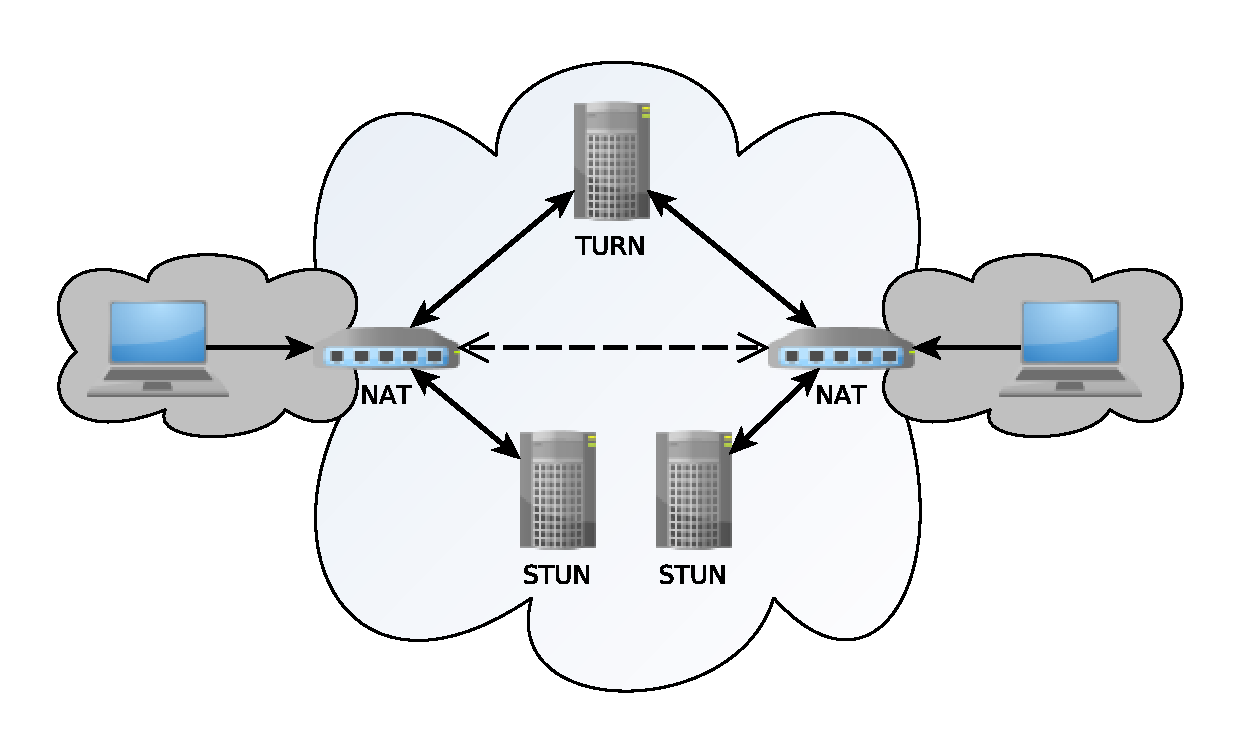
\includegraphics[width=0.55\textwidth]{figures/ice.pdf}
		\end{flushright}
		
		\end{frame}




	\subsection{Real-Time communications}\label{rtc}

		\begin{frame}[c]
		\frametitle{Real-Time communications}

		WebRTC (Web Real-Time Communications)

		\begin{itemize}
		\item Access to camera, microphone and screen*
		\item Peer to Peer file and stream sharing
		\item Standardized protocols
		\item No plug-ins required
		\end{itemize}

		\begin{flushright}

			\vspace*{-5\baselineskip}
			
\includegraphics[width=0.2\textwidth]{figures/webrtc.png}
		\end{flushright}
		
			\tiny{* requires installing a plug-in yet.}

		\end{frame}


		\begin{frame}[c]
		\frametitle{Real-Time communications}

\begin{table}[]
\centering
%\caption{My caption}
\label{my-label}
\begin{tabular}{cccc}
 \begin{minipage}{.2\textwidth}
\includegraphics[width=\linewidth]{figures/skype.png}\end{minipage} &  
 \begin{minipage}{.2\textwidth}
\includegraphics[width=\linewidth]{figures/hangouts.png}\end{minipage} &  
 \begin{minipage}{.2\textwidth}
\includegraphics[width=\linewidth]{figures/jitsi.png}\end{minipage} &  
 \begin{minipage}{.2\textwidth}
\includegraphics[width=\linewidth]{figures/kurento.png}\end{minipage} \\
Skype & Hangouts & Jitsi & Kurento   \\
\tiny Proprietary Application & \tiny WebRTC Application$^{*}$ & \tiny WebRTC Application \& Framework & \tiny WebRTC Framework  \\
\tiny Audio/Video/Text & \tiny Audio/Video/Text & \tiny Audio/Video/Text & \tiny Audio/Video  \\
\tiny File Sharing & \tiny Collaborative Tools & \tiny Collaborative Tools & \tiny Stream Recording 
\end{tabular}
\end{table}

	\tiny{* requires installing a plug-in on non chrome web browsers.}
		\end{frame}




%	\subsection{Signaling}
%  		\begin{frame}[c]
%		\frametitle{Signaling: meet and get to know}
%		\begin{itemize}
%		\item Own Implementation
%		\vfill
%		\item SIP
%		\vfill
%		\item XMPP
%		\vfill
%		\item SigOFly 
%		\end{itemize}
%		\end{frame}



	\subsection{Hypermedia}
  		\begin{frame}[c]
		\frametitle{Hypermedia: more than words, more than images}
		\begin{itemize}
		\item \textbf{Concepts:} HyperText \& HyperMedia \& HyperCommunications \& Detail on  Demand
		\vfill
		\item \textbf{Implementations:} HyperCafe \& HyperHitchcock  % Detail on Demand
				
		\end{itemize}
		
		\begin{figure}
			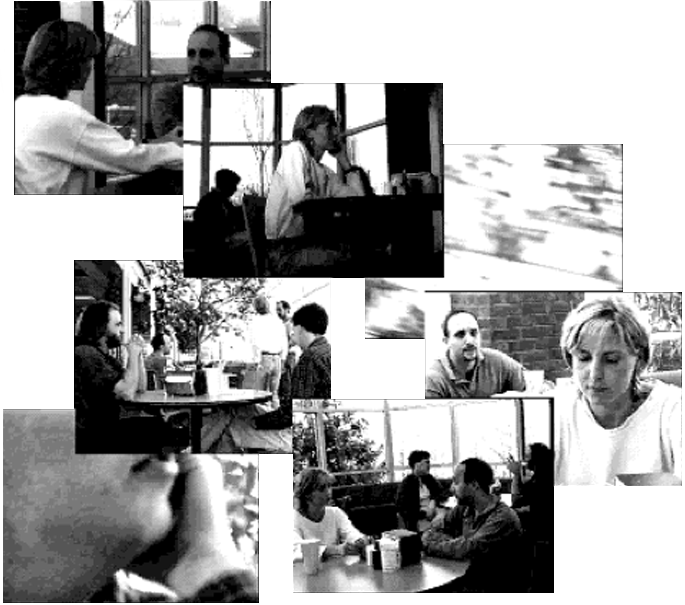
\includegraphics[height=0.4\textheight]{figures/hypercafe.png}
			
\includegraphics[height=0.1\textheight]{figures/space.png}
			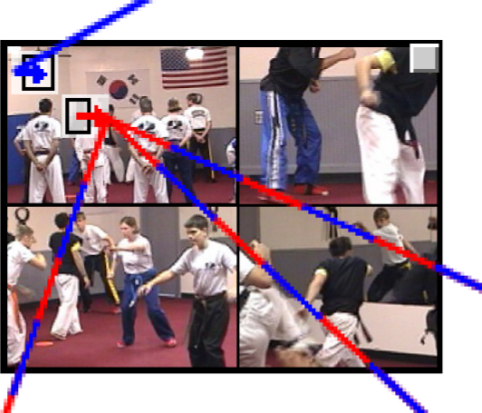
\includegraphics[height=0.4\textheight]{figures/hitchcock.png}
		\end{figure}
		\end{frame}


%		\begin{frame}[c]
%		\frametitle{Hypermedia: more than words, more than images}
%		\begin{itemize}		
%		\item \textbf{Languages:} HyVAL \& SMIL
%		\vfill
%		\item \textbf{WebBrowser:} Ambulant \& SmillingWeb \& SVG
%		\end{itemize}
%		
%		\begin{multicols}{2}
%		\begin{figure}
%			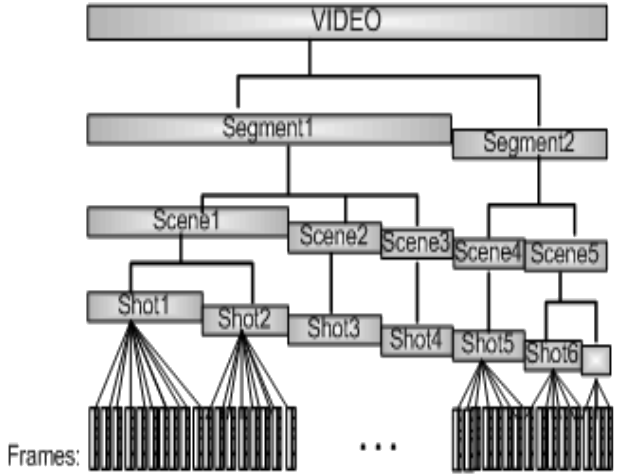
\includegraphics[height=0.4\textheight]{figures/hyval.png}
%			\caption{HyVAL structure}
%		\end{figure}
%		\begin{figure}
%			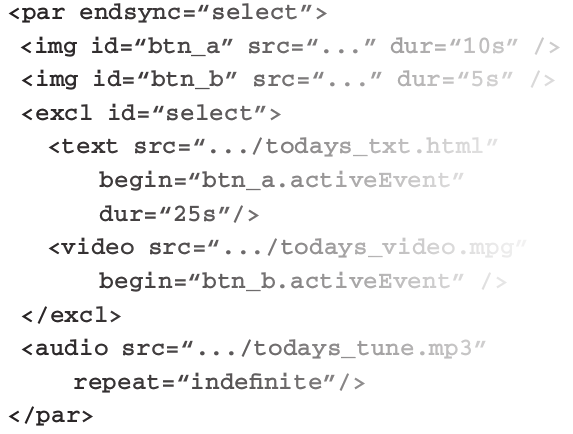
\includegraphics[height=0.4\textheight]{figures/smil.png}
%			\caption{SMIL example}
%		\end{figure}
%		\end{multicols}
%		\end{frame}


% 		\begin{frame}[c]
%		\frametitle{Web-Browser plug-ins}
%		\begin{figure}
%			
\includegraphics[height=0.3\textheight]{figures/flash.jpg}
%			
\includegraphics[height=0.1\textheight]{figures/space.png}
%			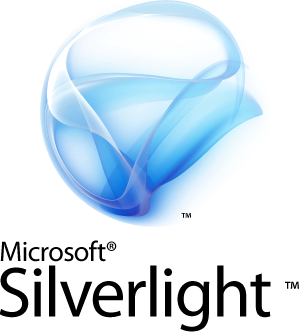
\includegraphics[height=0.3\textheight]{figures/silverlight.png}
%		\end{figure}
%		\end{frame}


	\subsection{Collaboration \& Time manipulation}
% 		\begin{frame}[c]
%		\frametitle{Extending collaboration tools with time manipulation}
%	
%		\begin{figure}
%			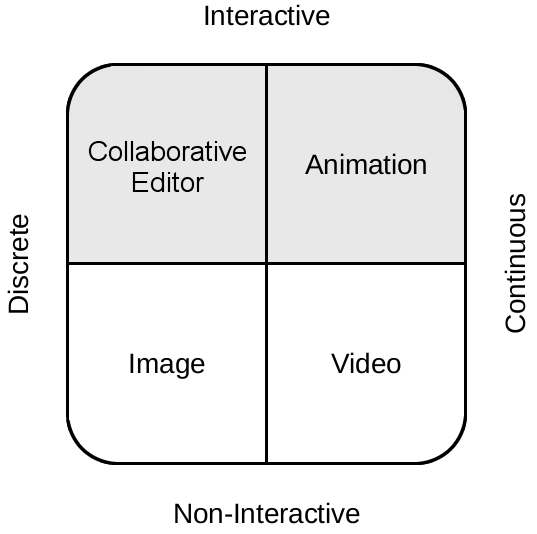
\includegraphics[height=0.5\textheight]{figures/media_types.png}
%			\caption{Media Types}
%		\end{figure}
%		\end{frame}



  		\begin{frame}[c]
		\frametitle{Extending collaboration tools with time manipulation}

			\begin{table}
			\centering
			\caption{Comparision between Operational Transformation libraries}
			\label{table:otcomparision}
			\begin{tabular}{|c|c|c|c|}
			\hline
			\textbf{Library} & \textbf{Own Server} & \textbf{Own Storage} & \textbf{Operations} \\ \hline
			ShareJS          & \cmark                 & \cmark                  & text+objects        \\ \hline
			TogetherJS       & \cmark                 & \xmark                   & text+objects        \\ \hline
			Goodow           & \cmark                 & \cmark                  & text+objects        \\ \hline
			Etherpad Lite    & \cmark                 & \cmark                  & extendable 			    \\ \hline
			OT.js            & \xmark                  & \xmark                   & text                \\ \hline
			\end{tabular}
			\end{table}

		\end{frame}

%\subsubsection{Streaming and Recording}\label{recstream}
%\subsubsection{Media Types}\label{mediatype}
%\subsubsection{Recording and Streaming Interactive Media}\label{intrecord}
%\subsubsection{Collaborative Environment}\label{collabenv}



\section{Architecture}\label{arch}

%\begin{frame}[t,shrink]
%\frametitle{Related Work} 
%\tableofcontents[currentsection,hideothersubsections]
%\end{frame}

\subsection{Modules}

	\begin{frame}[c]
		\frametitle{Modules}
		\begin{figure}[H]
			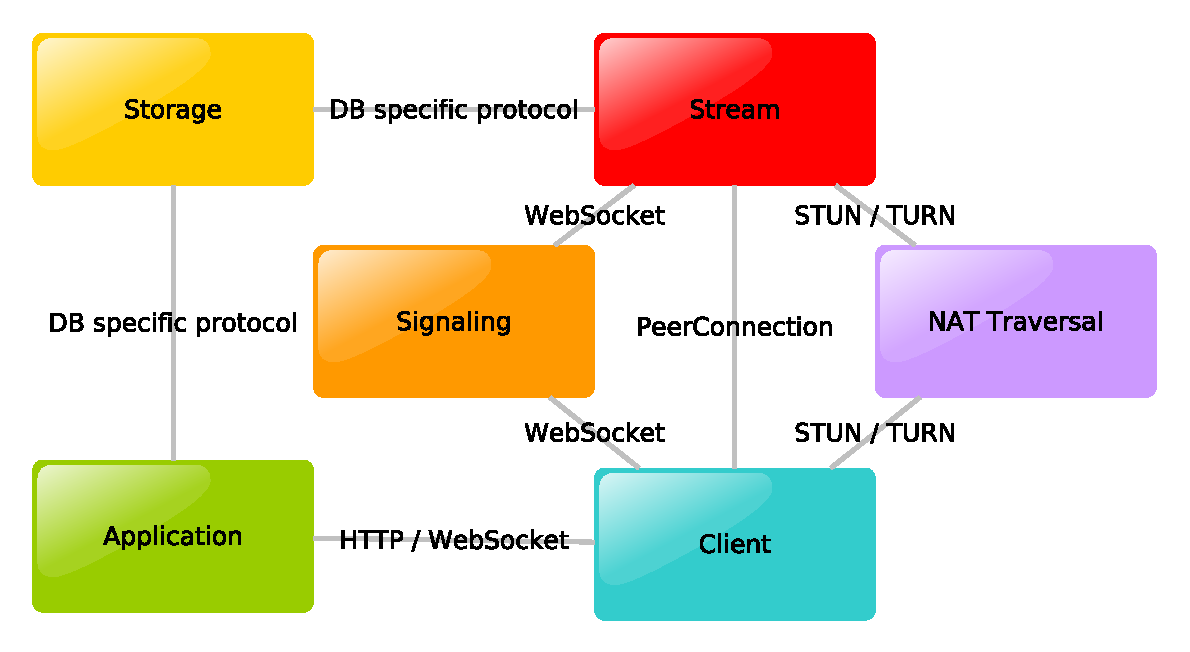
\includegraphics[width=0.8\textwidth]{figures/modules.pdf}
			\caption{System Modules}
		\end{figure}
	\end{frame}

\subsection{Implementation Proposal}

		\begin{frame}[c]
		\frametitle{System Infrastructure}



		\begin{figure}[H]
			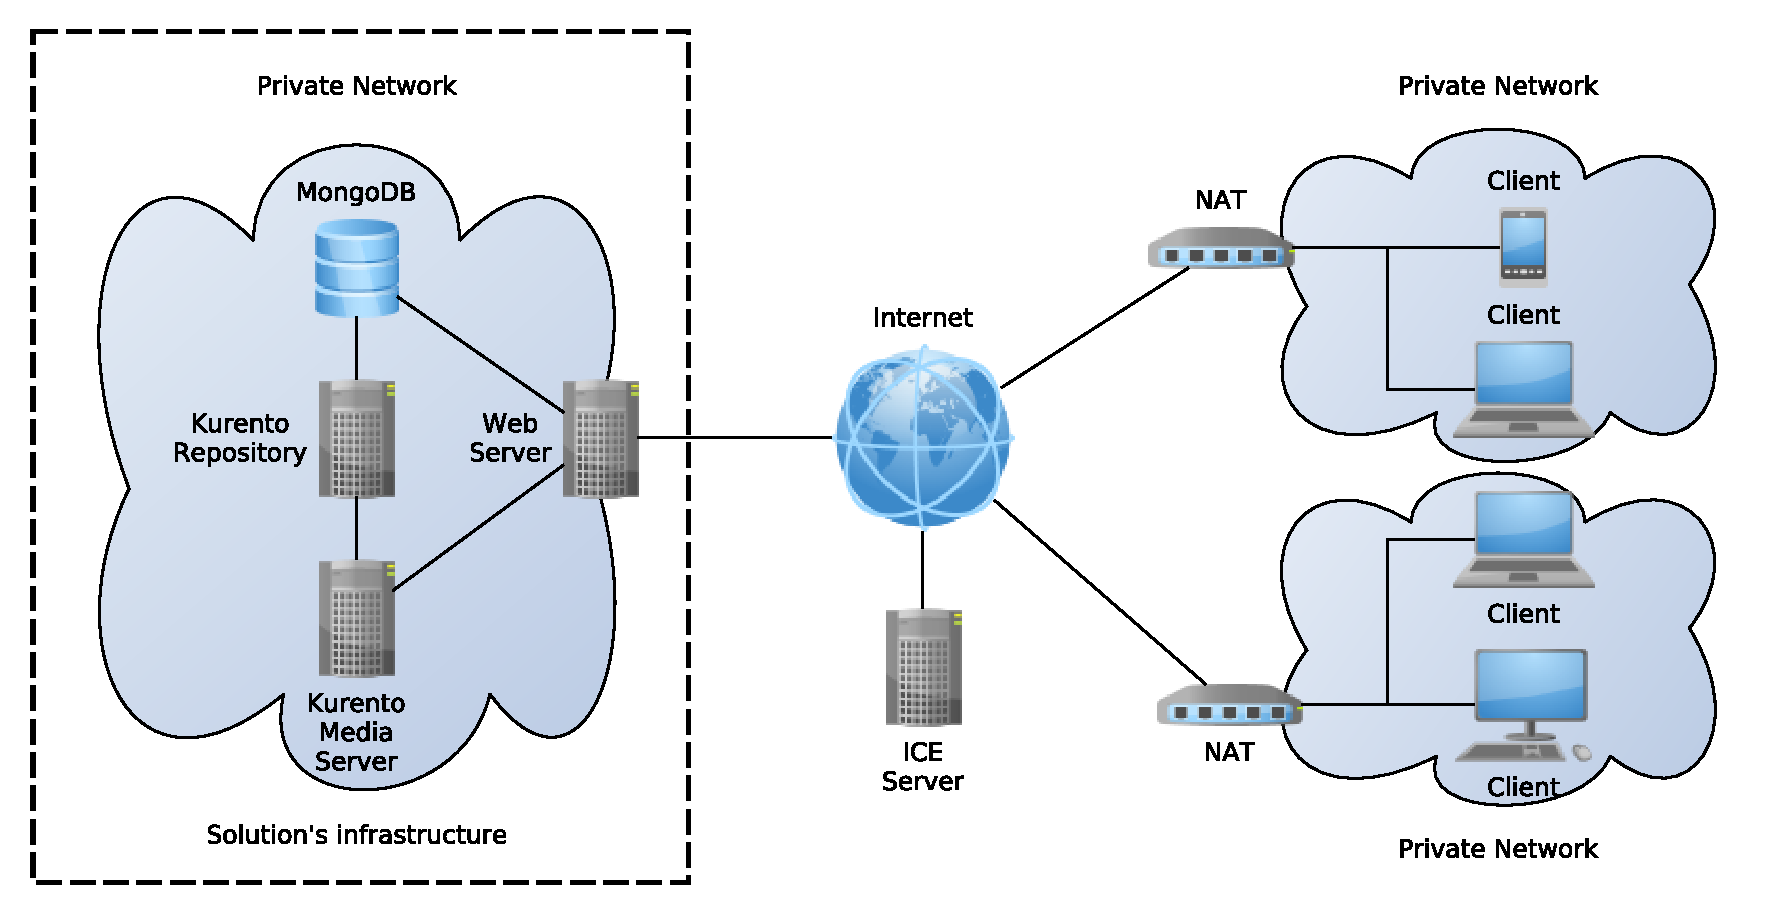
\includegraphics[width=0.9\textwidth]{figures/infrastructure.pdf}
			\caption{System Infrastructure}
		\end{figure}

\begin{itemize}
		\item \small \textbf{Signaling Server \& Web Server}: Play Framework
		\item \textbf{Stream Server}: Kurento Media Server		
		\item \textbf{Database}: MongoDB
		\end{itemize}




		\end{frame}

		\begin{frame}[c]

		\frametitle{Application Architecture}

\begin{table}[H]
\centering
	\caption{Application Architecture}
	\label{table:apparch}

	\resizebox{\textwidth}{!}{%
    \begin{tabular}{ccccccccc@{}m{0pt}@{}}
	\hline 
\multicolumn{9}{|c|}{\cellcolor{Gray}Application}  &\\[12pt]\cline{1-6}\cline{8-8}
\multicolumn{2}{|c|}{~~~~~jQuery~~~~~} & \multicolumn{1}{c|}{HTML5} & \multicolumn{1}{c|}{CSS3 (Bootstrap)} & \multicolumn{1}{c|}{Signaling} & \multicolumn{1}{c|}{~~~~~ot.js~~~~~} & \multicolumn{1}{c|}{\cellcolor{Gray}~~~~~~~~~~~~~~~} & \multicolumn{1}{c|}{adapter.js} &   \multicolumn{1}{c|}{\cellcolor{Gray}~~~~~~~~~~~~~~~} &\\[12pt]\hline
\multicolumn{1}{|c|}{HTTP} & \multicolumn{3}{c|}{User Interface}  & \multicolumn{3}{c|}{WebSocket}    & \multicolumn{2}{c|}{WebRTC}      &\\[12pt]\hline
\end{tabular}}
\end{table}


		\end{frame}


\section{Implementation}\label{meth} % Section
%\begin{frame}[t,shrink]
%\frametitle{Implementation} 
%\tableofcontents[currentsection,hideothersubsections]
%\end{frame}

\subsection{Signaling Protocol}
\begin{frame}[c]
		\frametitle{Signaling Protocol}
		\begin{figure}[H]
			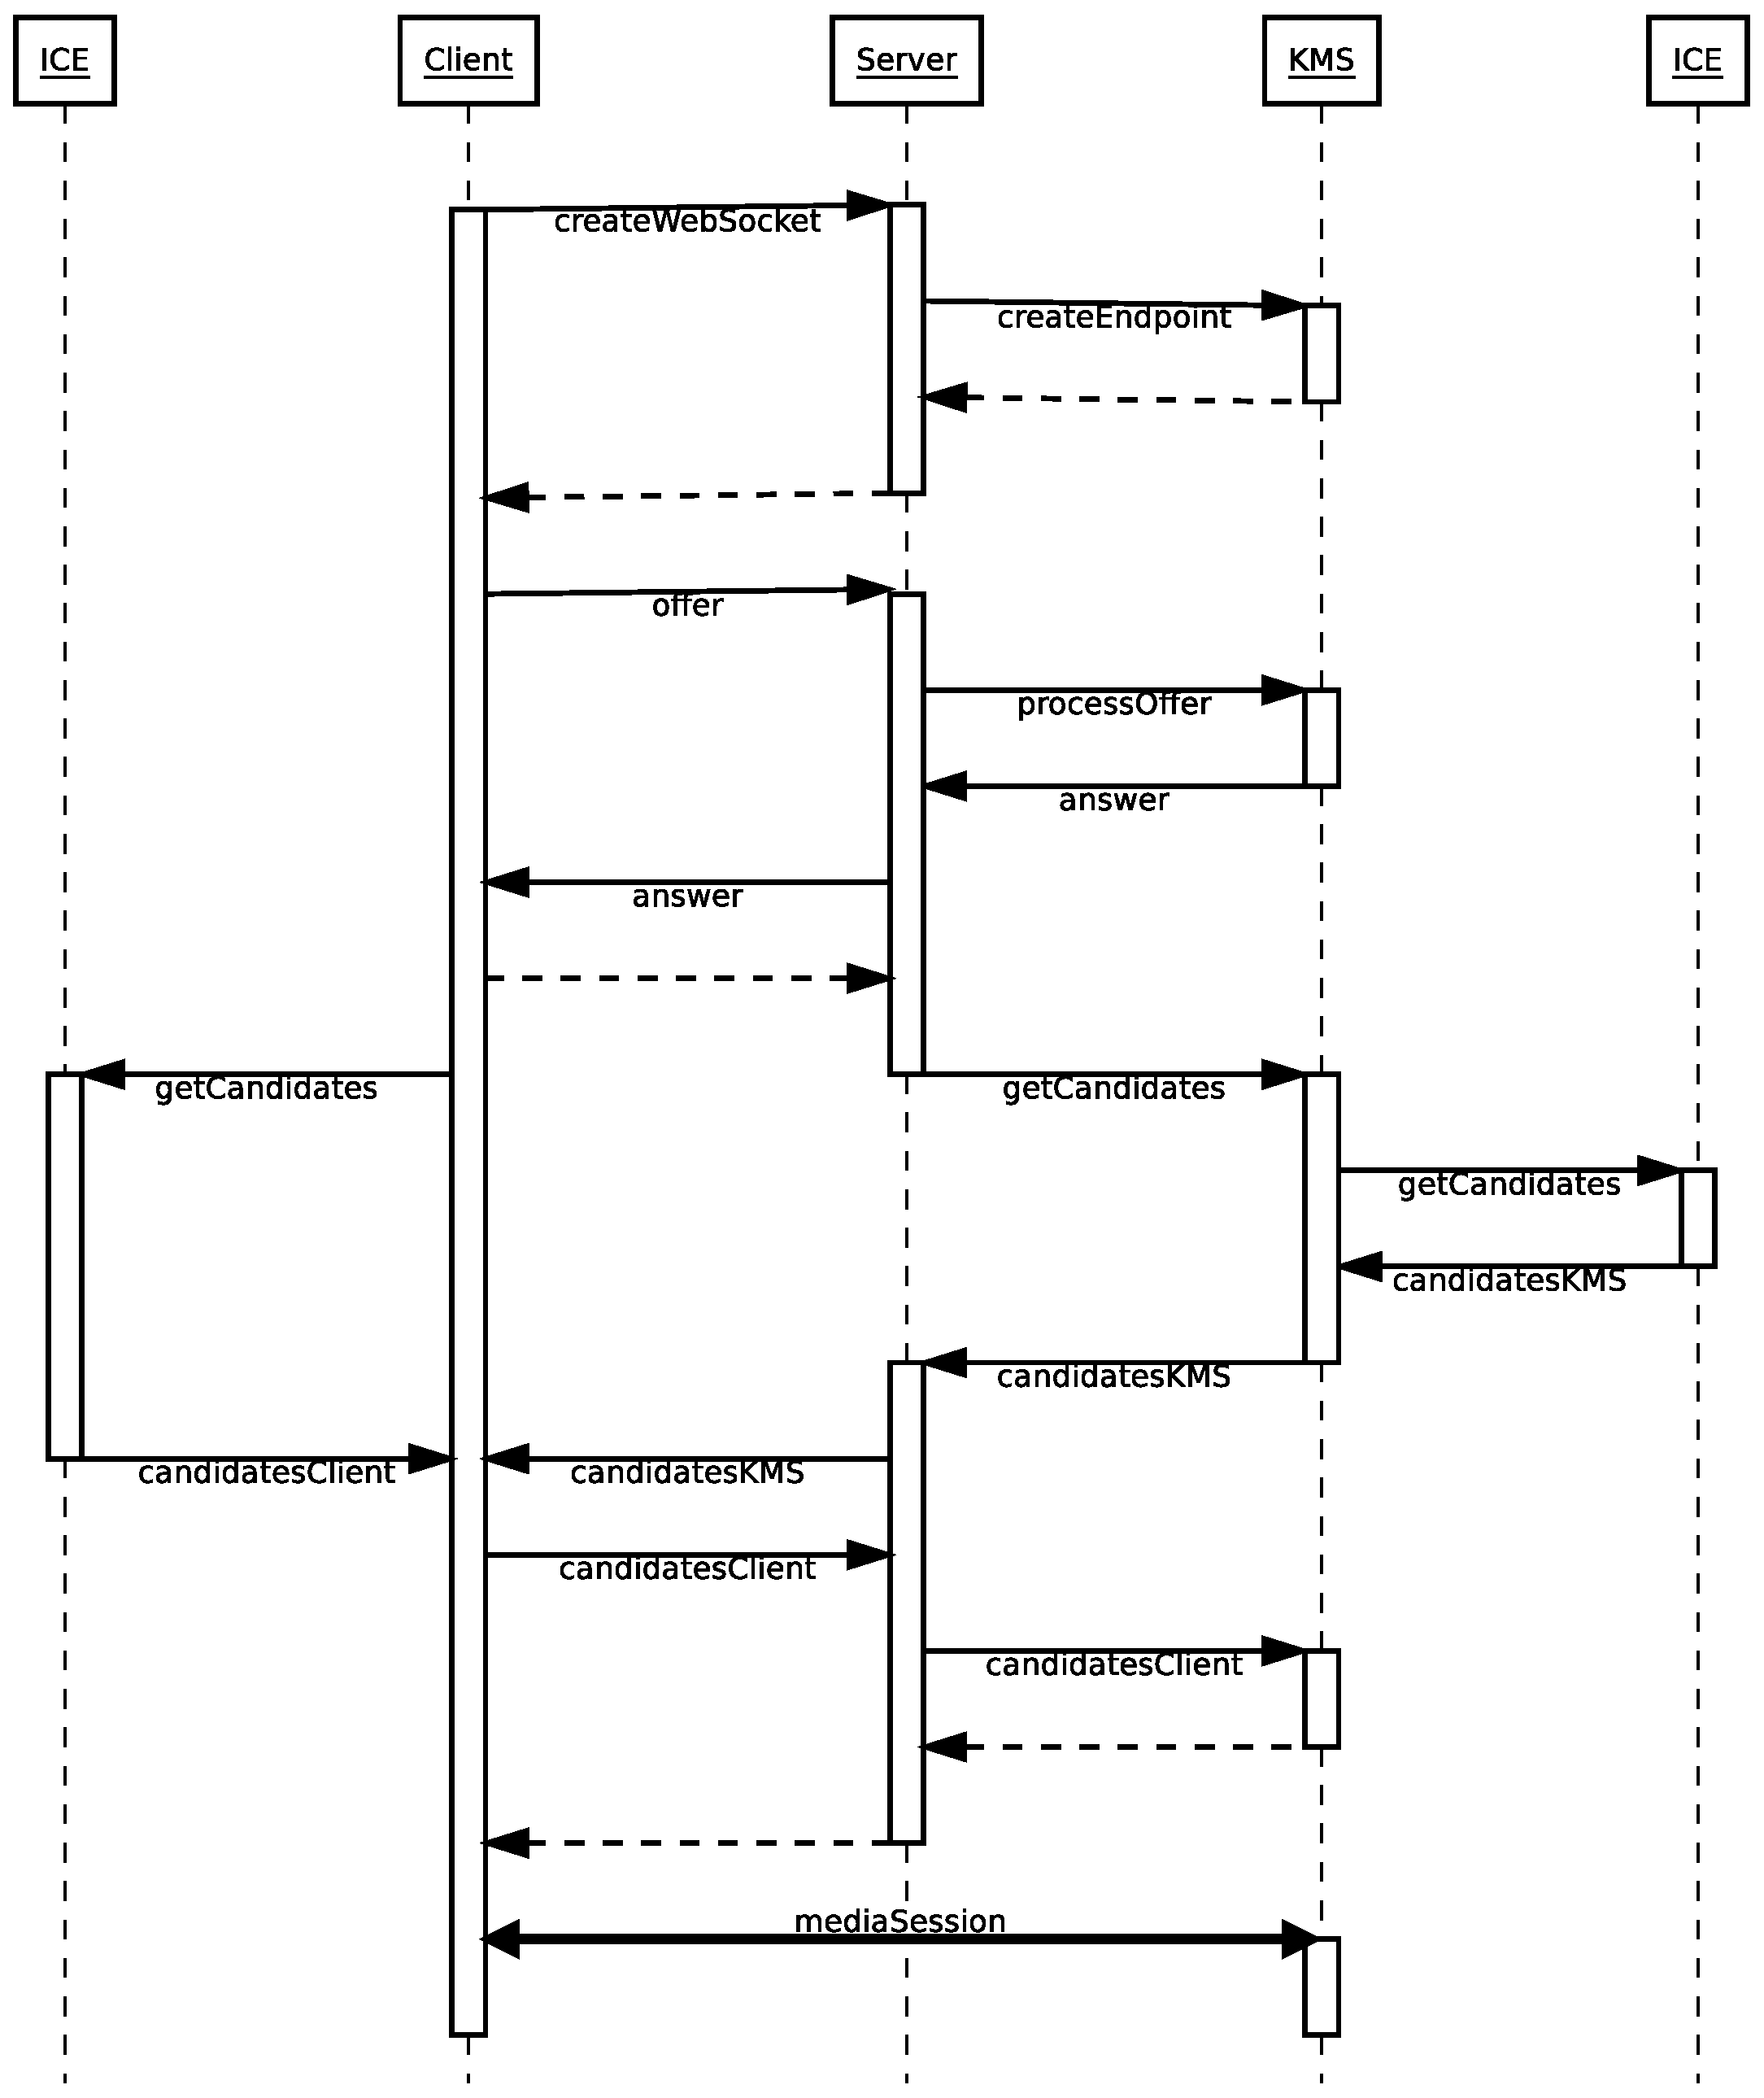
\includegraphics[width=0.55\textwidth]{figures/signaling.eps}
			\caption{Signaling Protocol}
		\end{figure}
\end{frame}



\subsection{Stream Recording}
\begin{frame}[c]
\centering
		\frametitle{Stream Recording}

		\begin{itemize}
\item Client-side recording.
		\vfill

\item Server-side recording to file system.
		\vfill

\item Server-side recording to database (Kurento Repository).
		\end{itemize}
	\end{frame}


\subsection{Stream composition}

		\begin{frame}[c]
		\frametitle{Stream composition}
		\begin{figure}
			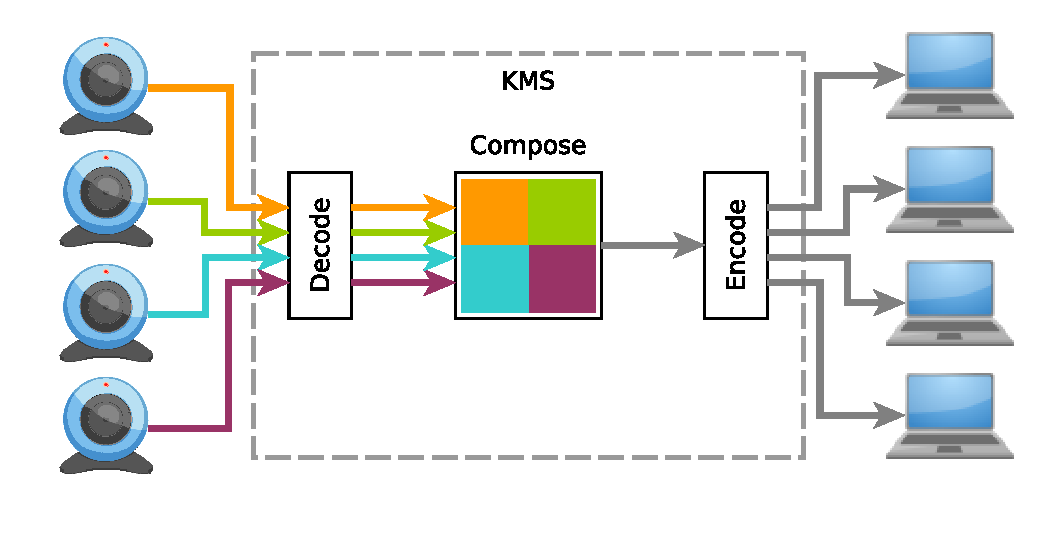
\includegraphics[width=0.5\textwidth]{figures/wcomposite.pdf}
			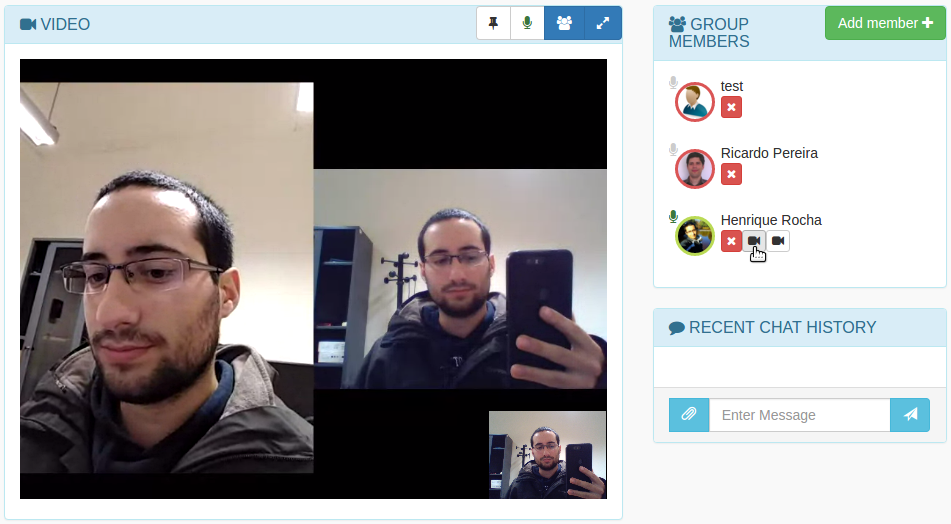
\includegraphics[width=0.5\textwidth]{figures/devices.png}
		\end{figure}
		\end{frame}


\subsection{Hyper-Content}

		\begin{frame}[c]
		\frametitle{Hyper-Content}


		\begin{itemize}
		\item Create \& Search content
				\vfill
\item Scheduler
		\vfill
		\item QR codes
		\vfill
		\item Security concerns
		\end{itemize}

		\begin{flushright}

			\vspace*{-11\baselineskip}
			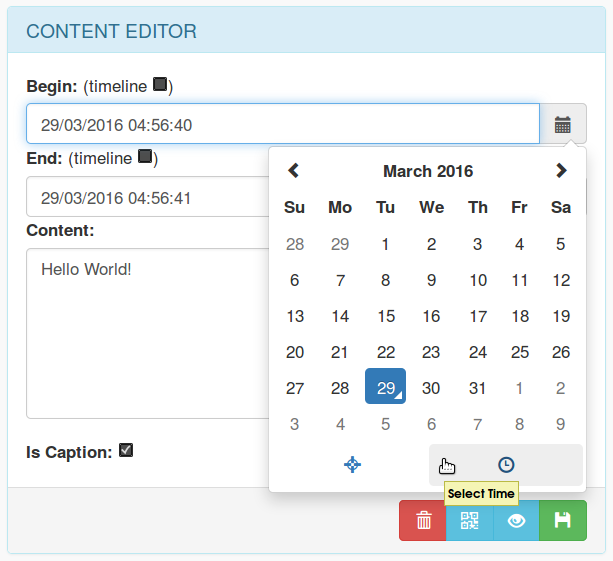
\includegraphics[width=0.5\textwidth]{figures/edition.png}
		\end{flushright}
		

		\end{frame}


\subsection{Time manipulation}

		\begin{frame}[c]
		\frametitle{Time manipulation}


		\begin{itemize}
		\item Playback recordings
		\item Create \& Search annotations
		\item Time Hyper-links
		\end{itemize}

			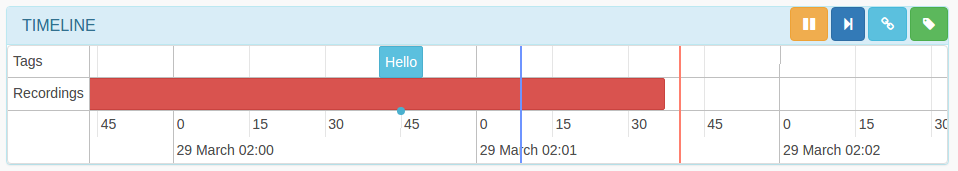
\includegraphics[width=\textwidth]{figures/timeline.png}
				\begin{flushright}

			\vspace*{-12\baselineskip}
			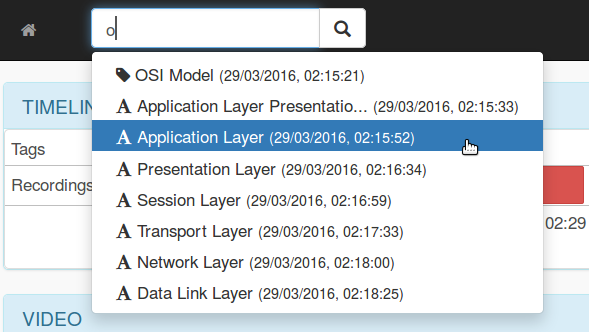
\includegraphics[width=0.45\textwidth]{figures/search.png}
		\end{flushright}
		

		\end{frame}


\subsection{Chat \& Collaborative environment}

		\begin{frame}[c]
		\frametitle{Chat \& Collaborative environment}


		\begin{itemize}
		\item Instant text messaging
			\begin{itemize}
			\item WebSockets
			\end{itemize}

		\item File sharing
			\begin{itemize}
			\item HTTP file upload
			\item stored in the database
			\end{itemize}
		
		\item Collaborative text editor (OT.js)
			\begin{itemize}
			\item retain
			\item insert
			\item delete
			\end{itemize}
		

		\end{itemize}
		

		\end{frame}




\section{Evaluation}\label{arch}

%\begin{frame}[t,shrink]
%\frametitle{Evaluation} 
%\tableofcontents[currentsection,hideothersubsections]
%\end{frame}

\subsection{Performance Tests}

	\begin{frame}[c]
		\frametitle{Performance Tests - CPU}
		\begin{figure}[H]
			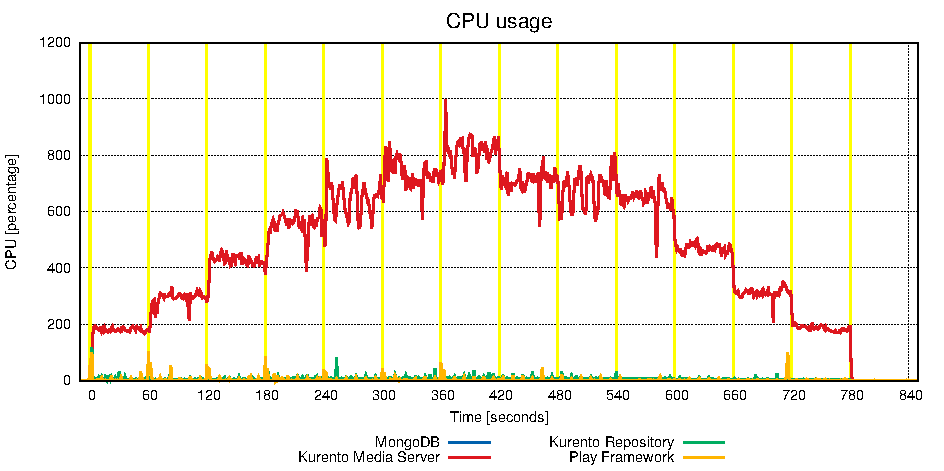
\includegraphics[width=\textwidth]{figures/cpu.pdf}
			\caption{CPU usage at server}
		\end{figure}
	\end{frame}
	\begin{frame}[c]
		\frametitle{Performance Tests - CPU (average)}
		\begin{figure}[H]
			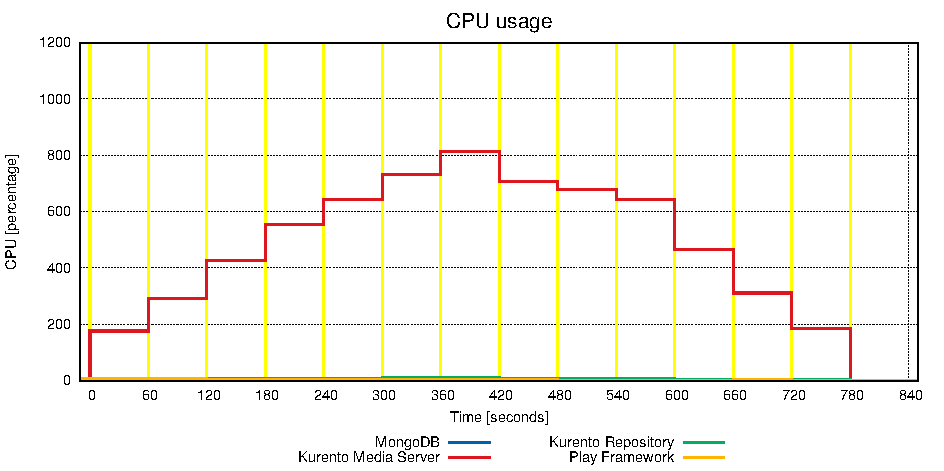
\includegraphics[width=\textwidth]{figures/cpu_avg.pdf}
			\caption{CPU usage at server (average per interval)}
		\end{figure}
	\end{frame}
	\begin{frame}[c]
		\frametitle{Performance Tests - Memory}
		\begin{figure}[H]
			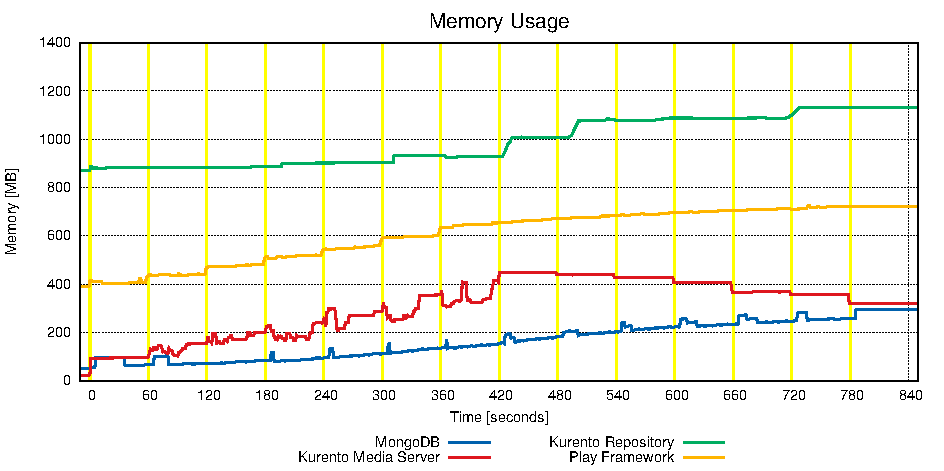
\includegraphics[width=\textwidth]{figures/ram.pdf}
			\caption{Memory usage at server}
		\end{figure}
	\end{frame}
	\begin{frame}[c]
		\frametitle{Performance Tests - Network Usage}
		\begin{figure}[H]
			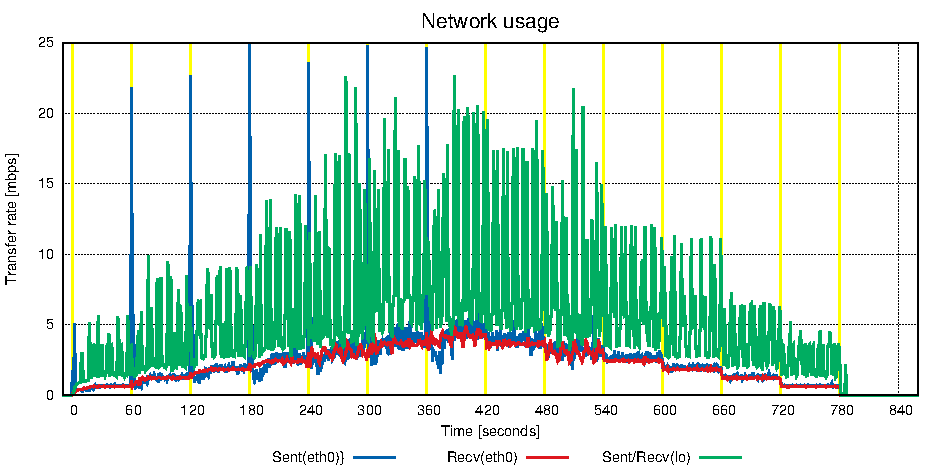
\includegraphics[width=\textwidth]{figures/net.pdf}
			\caption{Network usage at server}
		\end{figure}
	\end{frame}
	\begin{frame}[c]
		\frametitle{Performance Tests - Network Usage (average)}
		\begin{figure}[H]
			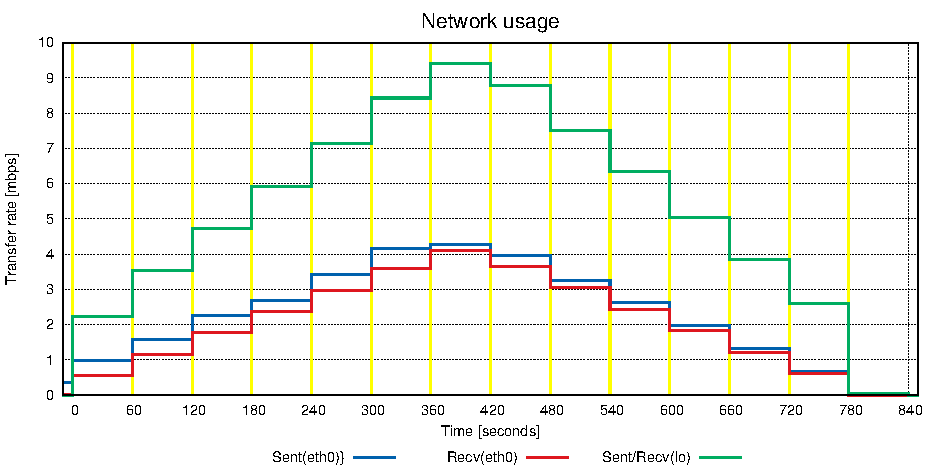
\includegraphics[width=\textwidth]{figures/net_avg.pdf}
			\caption{Network usage at server (average per interval)}
		\end{figure}
	\end{frame}
	\begin{frame}[c]
		\frametitle{Performance Tests - Network Usage}
		\begin{figure}[H]
			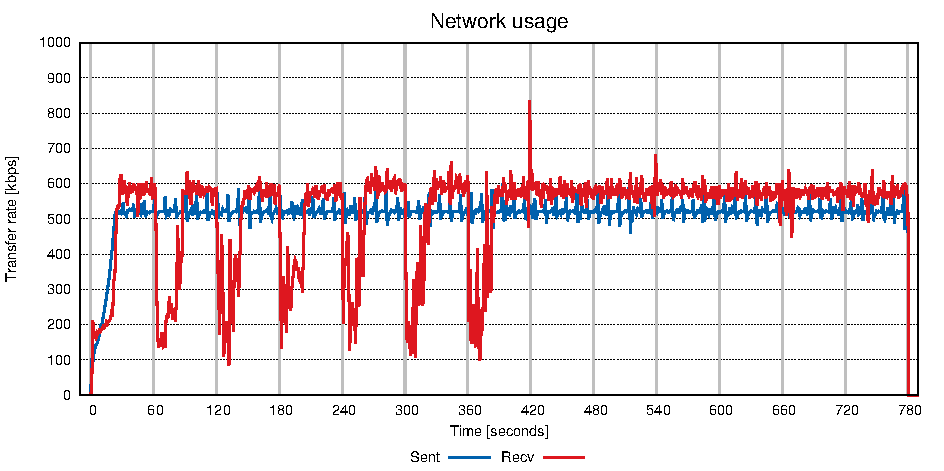
\includegraphics[width=\textwidth]{figures/net_clt.pdf}
			\caption{Network usage at client}
		\end{figure}
	\end{frame}

\subsection{User Interface Tests}

	\begin{frame}[c]
		\frametitle{User Interface Tests}
		\begin{figure}[H]
			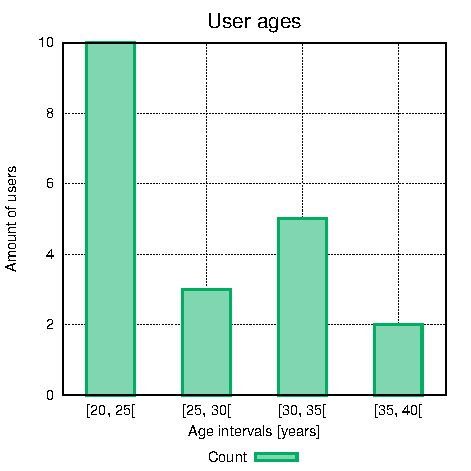
\includegraphics[width=0.5\textwidth]{figures/user_ages.pdf}
			\caption{Users age}
		\end{figure}
	\end{frame}
	\begin{frame}[c]
		\frametitle{Five tasks}
		\begin{figure}[H]
			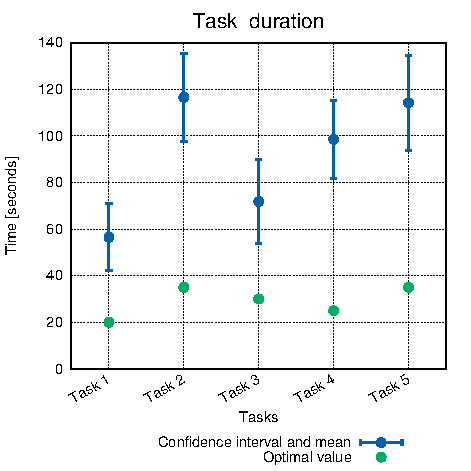
\includegraphics[width=0.5\textwidth]{figures/user_times.pdf}
			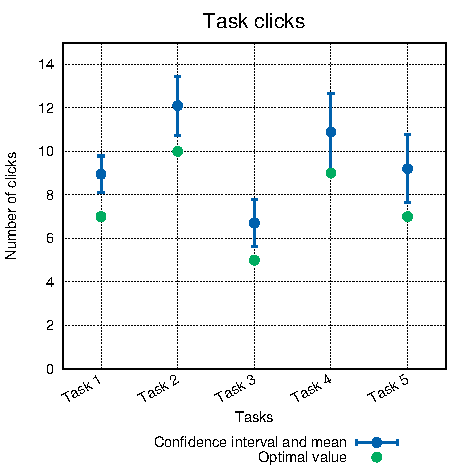
\includegraphics[width=0.5\textwidth]{figures/user_clicks.pdf}
			\caption{Tasks metrics}
		\end{figure}
		\begin{itemize}
			\item Difficulty per task.
			\item Errors per task.
		\end{itemize}
	\end{frame}
	\begin{frame}[c]
		\frametitle{Overall evaluation}
		\begin{figure}[H]
			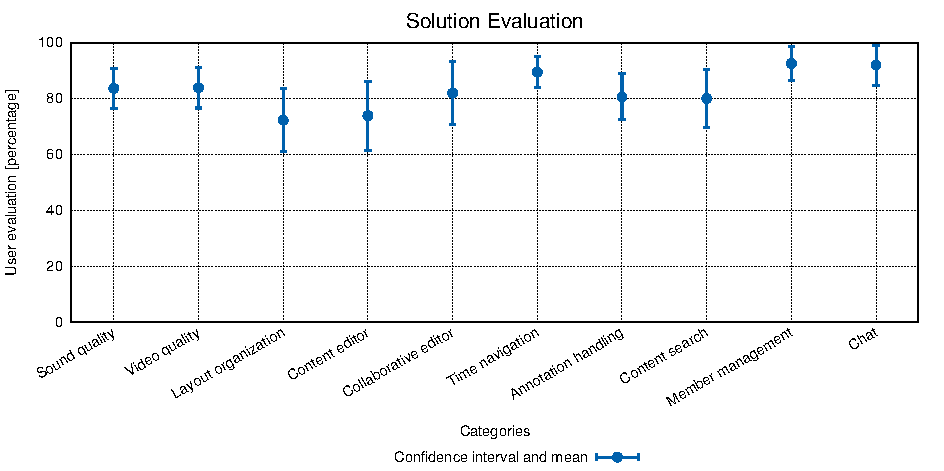
\includegraphics[width=\textwidth]{figures/user_evals.pdf}
			\caption{Overall evaluation}
		\end{figure}
	\end{frame}

\section{Conclusions}\label{concl} % English
%\begin{frame}[t,shrink]
%\frametitle{Related Work} 
%\tableofcontents[currentsection,hideothersubsections]
%\end{frame}

\begin{frame}[c]
		\frametitle{Conclusions}
		\begin{itemize}
\item New usage scenarios for communication and collaboration applications.
		\vfill

\item Enrich communications using hypermedia concepts. Record, playback and collaboration features.
		\vfill

\item Prototype implementation and testing.
		\end{itemize}

	\end{frame}

  		\begin{frame}[c]
		\frametitle{Demonstration}
		%A teacher record and streams an interactive class, some students participate in real-time others may participate later.
		%\vfill
		%The teacher adds information to its class (create tags, add links, overlay images ...).
		%\vfill
		%Students can answer to quizzes.
	
		\begin{center}
		\href{run:video.mp4}{
		
\includegraphics[scale=0.25]
		{video.eps}}
		\end{center}


		\end{frame}

\section{Future Work}\label{concl} % English
%\begin{frame}[t,shrink]
%\frametitle{Related Work} 
%\tableofcontents[currentsection,hideothersubsections]
%\end{frame}

\begin{frame}[c]
		\frametitle{Future Work}
		\begin{itemize}
\item Implement fast-forward playback.
		\vfill

\item Improve solution's security.
		\vfill

\item Scale our solution to multiple servers.
		\end{itemize}

	\end{frame}



%------------------------------------------------

%------------------------------------------------

%------------------------------------------------

\begin{frame}[c]
\Huge{\centerline{Questions?}}
\end{frame}

%----------------------------------------------------------------------------------------

\end{document} 
